\documentclass{article}


\usepackage{PRIMEarxiv}

\usepackage[utf8]{inputenc} % allow utf-8 input
\usepackage[T1]{fontenc}    % use 8-bit T1 fonts
\usepackage{bbm}            % mathbb for digits
\usepackage{hyperref}       % hyperlinks
\usepackage{url}            % simple URL typesetting
\usepackage{booktabs}       % professional-quality tables
\usepackage{amsfonts}       % blackboard math symbols
\usepackage{nicefrac}       % compact symbols for 1/2, etc.
\usepackage{microtype}      % microtypography
\usepackage{amsmath}        % Aligned
\usepackage{lipsum}
\usepackage{fancyhdr}       % header
\usepackage{graphicx}       % graphics
\usepackage{tikz}           % Load TikZ package
\usepackage{ifthen}         % 
\usepackage{siunitx}        % For better numerical alignment
\usepackage{caption}        % For improved caption formatting
\graphicspath{{media/}}     % organize your images and other figures under media/ folder

%Header
\pagestyle{fancy}
\thispagestyle{empty}
\rhead{ \textit{ }} 

% Update your Headers here
% \fancyhead[LO]{Running Title for Header}
% \fancyhead[RE]{Firstauthor and Secondauthor} % Firstauthor et al. if more than 2 - must use \documentclass[twoside]{article}



  
%% Title
\title{SICK BIDE: Softmax Implicit Compute Kernel allows Binary Implicit Distribution Encoding
%%%% Cite as
%%%% Update your official citation here when published 
% \thanks{\textit{\underline{Citation}}: 
% \textbf{Authors. Title. Pages.... DOI:000000/11111.}} 
}

\author{
  Théo Boyer \\
  Duon Labs \\
  \texttt{theo@duonlabs.com} \\
  %% examples of more authors
   \And
  Santiago Malter-Terrada \\
  Duon Labs \\
  \texttt{santi@duonlabs.com} \\
}


\begin{document}

\setlength{\tabcolsep}{5pt} % Reduce column spacing
\renewcommand{\arraystretch}{1.2} % Increase row spacing

\maketitle


\begin{abstract}
Deep learning has achieved remarkable progress by minimizing domain-specific assumptions in favor of data-driven learning. In this paper, we introduce the Binary Implicit Distribution Encoding (BIDE), a novel framework for assumption-free distribution modeling that unifies continuous, categorical, and ordered distributions. By leveraging binary representations, BIDE implicitly encodes probability distributions without relying on predefined structures.

Complementing BIDE is the Softmax Integral Compute Kernel (SICK), a GPU kernel for efficiently computing softmax normalization over combinatorial binary spaces, addressing the computational challenges of this approach. Together, BIDE and SICK form a scalable, memory-efficient, and expressive alternative for generative modeling, probabilistic inference, and large language models (LLMs).

Experimental results demonstrate BIDE's ability to accurately model complex distributions without prior knowledge, highlighting its potential to redefine distribution modeling. This framework opens new avenues for generative AI, probabilistic forecasting, and other applications requiring flexible and assumption-free distribution representations.
\end{abstract}


% keywords can be removed
\keywords{Probabilistic Modeling \and Implicit Representations \and GPU kernel}


\section{Introduction}
Modeling distributions is a cornerstone of machine learning, especially in the deep learning based generative era with countless applications as diverse as natural language processing (NLP), Image / Video generation or time series. While categorical distributions can be trivially addressed, continuous distributions are not as trivial. Traditionally, two classes of approaches dominate continuous distribution modeling: parametric modeling, which requires \textit{a priori} knowledge about distributions family, and discretization, which maps continuous spaces into discrete ones. While these methods have proven effective in many contexts, they are often constrained by their inherent trade-offs in flexibility, expressiveness, and computational efficiency. Furthermore, deep learning has consistently improved as the methods were more general and carried less assumptions about the problems it solves (\cite{Silver2017}, \cite{vaswani2017attention})

Binary Implicit Distribution Encoding (BIDE) introduces a paradigm shift in how we approach distribution modeling. By directly leveraging binary representations of data, BIDE provides a unified framework to model continuous, categorical, and ordered distributions. Instead of relying on approximations or domain-specific assumptions, BIDE maps binary inputs to their likelihood logits using a lightweight neural network architecture, allowing for expressive and memory-efficient implicit distribution representations.

Complementing BIDE is the Softmax Integral Compute Kernel (SICK), a GPU-optimized kernel designed to compute the softmax denominator and gradients required for BIDE's operation. In the same spirit as FlashAttention\cite{dao2022flashattention} SICK’s method of denominator computation ensures exact computation without materializing the full intermediate representations. Without this kernel, materializing the $2^n$ binary combinations and their intermediate computations would not be feasible because of both compute and memory bottlenecks, especially for high values of $n$.

This paper explores the design, implementation, and implications of the BIDE and SICK framework. We focus on the key use case of modeling continuous distributions without assumptions in a way that combines the expressiveness of categorical approaches with the flexibility of continuous methods. We demonstrate BIDE's ability to correctly approximate continuous distributions and SICK's significant improvements in memory efficiency and computational throughput.

To evaluate the viability of this framework, we present a thorough theoretical analysis of the computational and memory requirements of SICK under two variants. This is followed by experimental results of our implementation of SICK, showcasing the effectiveness of the 2 declinations. The findings underline the potential of BIDE and SICK as a transformative tool for distribution modeling, with applications extending to language modeling, probabilistic inference, and beyond.

This work contributes:

\begin{itemize}
\item A novel approach to distribution modeling: BIDE leverages binary representations to unify and extend traditional modeling paradigms.
\item GPU-optimized computation: SICK efficiently handles normalization and gradient calculations.
\item Insights into scalability and practicality: Through theoretical analysis and experimental validation, we highlight the trade-offs and potential optimizations of this framework.
\end{itemize}
The remainder of the paper is structured as follows. Section 2 provides background on distribution modeling and GPU optimizations. Section 3 details the methodology behind BIDE and SICK, including their architectural design and mathematical underpinnings. Section 4 presents experimental results and applications. Section 6 discusses the implications and limitations of the framework, and Section 7 concludes with future directions.


\section{Background}

\subsection{Distribution Modeling}
Modeling data distributions is a cornerstone of statistical and machine learning methods. Continuous distributions are often approximated using parametric models, such as Gaussian distributions or mixture of distributions, or discretized to apply categorical methods. While these approaches are computationally cheap, they both impose limitations on the flexibility and expressiveness of the modeled distributions. As a consequence their predictive performances directly depend on the correctness of the hypotheses made by the model developers which prevents any form of assumption-free prediction.

Recent advances in neural networks such as normalizing flows \cite{rezende2016variationalinferencenormalizingflow} have extended the ability to model complex, high-dimensional distributions. However, these approaches often come with trade-offs like memory and computational overhead, or constraints on the model architecture. Furthermore they are not completely assumption-free.

\subsection{Challenges in Categorical Distribution Modeling with neural networks}
Predicting a distribution over a categorical set using a neural network is a trivial problem as one just needs to apply a layer with its output dimensions being equal to the size of the set. While this is a viable approach for reasonable set sizes, it has two significant drawbacks when scaling to big numbers:
\begin{itemize}
\item The memory consumption of the weight of the output scales linearly with the set size. This directly impact Large models that also have a large hidden dimension, leading to huge weights of $O(ND)$. And it also impacts small models that target a big set, as the computation of the output layer dominates the ressources consumption of the total forward pass of the model.
\item The states that are rare in the training set can cause problems as their associated weights are pushed towards zero \cite{land2024fishingmagikarp}. A way to mitigate this problem would be to leverage structure between states for extrapolation.
\end{itemize}
The LLMs vocab size being constently growing, even reaching $256K$ for Gemma \cite{gemmateam2024gemma} we believe that any alternative methods that describe categorical distributions over big sets could be relevant in the future.

\subsection{GPU Optimizations in Neural Computation}
GPUs have become essential for accelerating deep learning workloads, offering massive parallelism and high memory bandwidth. Modern GPU programming frameworks, such as Triton and CUDA, enable fine-grained control over kernel-level operations. Leveraging these frameworks, researchers have developed optimized implementations for key operations like matrix multiplications, activation functions, and attention layer \cite{dao2022flashattention}.

Using a vanilla deep learning framework like Pytorch \cite{paszke2019pytorch} allow researchers and developers to utilize quite well the GPUs. However applying sequentially one kernel per operation is often suboptimal because of repeated memory transfers. Some features such as compilation allow for automated kernel fusion, increasing the GPU effectiveness. However compilers fail to optimize complex operations that require a mathematical rewrite of the formulas. As a consequence neural network layer kernels are still an active area of research \cite{dao2022flashattention} \cite{dao2023flashattention2}\cite{shah2024flashattention3}\cite{gu2024mamba}.
This is also why intermediary DSL like triton \cite{tillet2019triton} were created to simplify the process of writing custom GPU kernels for complex neural network layers.

\subsection{Binary Implicit Distribution Encoding and Softmax Integral Compute Kernel}
The Binary Implicit Distribution Encoding (BIDE) introduces a novel neural network layer that models distributions directly from binary representations of data. Unlike traditional embedding methods, BIDE can efficiently map inputs to logits by leveraging their binary representations, and making it well-suited for applications like continuous distribution modeling and memory-efficient vocabulary distributions in LLMs.

The Softmax Integral Compute Kernel (SICK) complements BIDE by providing GPU-optimized implementations for forward and backward computations. SICK leverages GPU kernels to compute the deniminator for the softmax operation with exact computation. This is achieved by exploiting GPU parallelism, binary operations, memory-aware block-wise computation, tiling and the online-softmax algorithm \cite{milakov2018onlinesoftmax}.

Together, BIDE and SICK address the limitations of existing methods by combining the expressiveness of categorical distributions with the precision of continuous models, all while optimizing for modern GPU hardware.

\section{Methodology}

\subsection{BIDE: Binary Implicit Distribution Encoding}
Binary Implicit Distribution Encoding (BIDE) is a novel neural network layer designed to model distributions over arbitrary inputs. The layer takes as input a binary representation of any data types, such as numbers (e.g., float16) or categories (e.g., uint16), and predicts their likelihood logits. This binary representation enables BIDE to generalize across data types with no modifications while maintaining computational efficiency.

\subsubsection{Architecture}
The BIDE layer is 1 hidden layer MLP. The input value is converted to its binary representation and mapped to $-1$ for zeros and $1$ for ones. Afterwards, we apply the input layer of the MLP with a gemm on the input vector followed by a ReLU. Finally, the output layer is applied again with a gemm outputing one value as the logit.

\subsubsection{Applications}
\begin{itemize} 
\item Continuous distributions: Unlike traditional methods that discretize continuous spaces or rely on parametric distributions, BIDE offers a flexible framework that combines expressiveness with computational tractability.
\item Memory-efficient vocabulary distributions: BIDE can replace conventional embeddings in large language models (LLMs), reducing memory overhead without compromising performance.
\item Tokenizer-free LLMs: Some tokenizer-free methods already exists by directly mapping input bytes to output bytes \cite{xue2022byt5}\cite{meta2024bytelatenttransformer} and lead to slower inference as more bytes are needed to express the equivalent of a token. BIDE would allow a native way to combine bytes together without architectural wrappers, either replacing the need for byte patching or being used on top of it.
\item Probabilistic Foundation model for time series: The assumption-free approach that SICK BIDE provides allow the creation of a new class of foundation models for time series based on probabilistic modeling and going beyond single point forecasts \cite{Garza2023timegpt} with a-posteriori uncertainty estimation methods like conformal prediciton \cite{angelopoulos2022gentleintroductionconformalprediction} and allow for a better expressivity than probabilistic models based on mixtures of distributions \cite{woo2024unifiedtraininguniversaltime}
\end{itemize}

\subsection{SICK: Softmax Integral Compute Kernel}
Softmax Integral Compute Kernel (SICK) is a GPU-optimized component that computes the normalization constants required for BIDE. Naïve numerically-stable softmax computation involves multiple passes over the logits, which can be computationally expensive when dealing with the $2^n$ binary combinations of $n$-bit inputs. But it's possible to compute it using the online softmax algorithm \cite{milakov2018onlinesoftmax}, with only one pass, and without the need to materialize the entire logits vector in memory.

\subsubsection{Forward Computation}
SICK performs computations of the softmax normalization constant by combining multiples tricks:
\begin{itemize}
\item Mixed precision: Some computations such as the gemm can be made in lower precisions with minimal loss of precision
\item Fused operation: Not materializing intermediates tensors in memory to avoid the peak memory bottleneck.
\item On-device input generation (brute-force variant): The binary nature of BIDE's inputs allows for generation of inputs on-device instead of generating the inputs on the host and transfer them. The memory transfer economy is significant as it's often the bottleneck of modern workloads.
\item Pre-computation trick (precomputed variant): It's possible to rewrite the formula of $z$ to turn the workload from the compute bounded regime to the memory bounded one. More details in \ref{method_pre_coputation}
\end{itemize}

\subsection{Fusion of SICK and cross-entropy loss}
\subsubsection{Forward Computation}
For the forward pass of the fused cross entropy loss, we simply evaluate BIDE with the labels $y$ and use SICK to compute the normalization constant. There is no need to develop a edicated kernel for this operation.

\subsubsection{Backward Computation}
The backward pass of BIDE is a classical MLP backward pass, and the main difficulty is the same as SICK's forward computation, which is iterating over the full combinatorial input space.
We show in appendix \ref{appendix_backward_pass} that it's possible to compute the most part of the gradient in the forward pass, with the formulas becoming:
\begin{align}
    \frac{\partial \mathcal{L}}{\partial r_i} &= \frac{1}{s} \sum_{k=1}^{K} h_{ki} \exp(l_k - m) - \frac{1}{N} \sum_{n=1}^{N} h_{y_ni} \\
    \frac{\partial \mathcal{L}}{\partial W_{ij}} &= \frac{1}{s} \sum_{k=1}^{K} b_{kj} \mathbbm{1}_{h_{ki} > 0} r_i \exp(l_k - m) - \frac{1}{N} \sum_{n=1}^{N} b_{y_nj} \mathbbm{1}_{h_{y_ni} > 0} r_i
\end{align}
Note that the loop over $K$ can be done in the forward pass as it doesn't depend on $y$.

\subsection{Hierarchical Pre-Computation for Efficiency} \label{method_pre_coputation}
We present the rewrite of the $z$ formula that allows to significantly reduce the compute capacity needed to achieve our objective.
Let's isolate one neuron of the hidden layer whoes pre-activation value $z$ is computed as such:

\begin{figure}[ht]
    \centering
    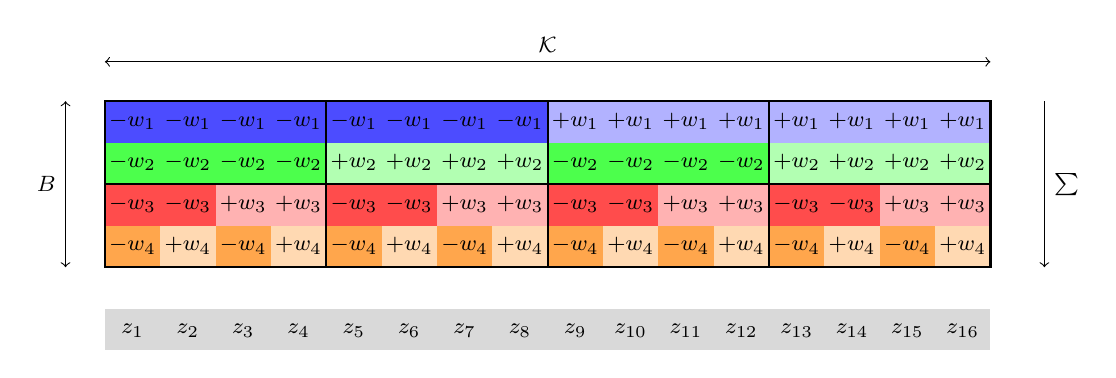
\begin{tikzpicture}[font=\footnotesize]
    \def\cw{2em}
    \def\ch{1.5em}
    
    \tikzset{cell/.style={
        inner sep=0pt,
        outer sep=0pt,
        minimum width=\cw,
        minimum height=\ch,
        align=center,
        text height=1ex,
        text depth=0.25ex,
        anchor=north west
    }}
    
    % w1 row (b=1, top)
    \node[cell, fill=blue!70]   at (0*\cw,0*\ch) {$-w_1$};
    \node[cell, fill=blue!70]   at (1*\cw,0*\ch) {$-w_1$};
    \node[cell, fill=blue!70]   at (2*\cw,0*\ch) {$-w_1$};
    \node[cell, fill=blue!70]   at (3*\cw,0*\ch) {$-w_1$};
    \node[cell, fill=blue!70]   at (4*\cw,0*\ch) {$-w_1$};
    \node[cell, fill=blue!70]   at (5*\cw,0*\ch) {$-w_1$};
    \node[cell, fill=blue!70]   at (6*\cw,0*\ch) {$-w_1$};
    \node[cell, fill=blue!70]   at (7*\cw,0*\ch) {$-w_1$};
    \node[cell, fill=blue!30]   at (8*\cw,0*\ch)  {$+w_1$};
    \node[cell, fill=blue!30]   at (9*\cw,0*\ch)  {$+w_1$};
    \node[cell, fill=blue!30]   at (10*\cw,0*\ch) {$+w_1$};
    \node[cell, fill=blue!30]   at (11*\cw,0*\ch) {$+w_1$};
    \node[cell, fill=blue!30]   at (12*\cw,0*\ch) {$+w_1$};
    \node[cell, fill=blue!30]   at (13*\cw,0*\ch) {$+w_1$};
    \node[cell, fill=blue!30]   at (14*\cw,0*\ch) {$+w_1$};
    \node[cell, fill=blue!30]   at (15*\cw,0*\ch) {$+w_1$};
    
    % w2 row (b=2)
    \node[cell, fill=green!70]  at (0*\cw,-1*\ch) {$-w_2$};
    \node[cell, fill=green!70]  at (1*\cw,-1*\ch) {$-w_2$};
    \node[cell, fill=green!70]  at (2*\cw,-1*\ch) {$-w_2$};
    \node[cell, fill=green!70]  at (3*\cw,-1*\ch) {$-w_2$};
    \node[cell, fill=green!30]  at (4*\cw,-1*\ch) {$+w_2$};
    \node[cell, fill=green!30]  at (5*\cw,-1*\ch) {$+w_2$};
    \node[cell, fill=green!30]  at (6*\cw,-1*\ch) {$+w_2$};
    \node[cell, fill=green!30]  at (7*\cw,-1*\ch) {$+w_2$};
    \node[cell, fill=green!70]  at (8*\cw,-1*\ch) {$-w_2$};
    \node[cell, fill=green!70]  at (9*\cw,-1*\ch) {$-w_2$};
    \node[cell, fill=green!70]  at (10*\cw,-1*\ch) {$-w_2$};
    \node[cell, fill=green!70]  at (11*\cw,-1*\ch) {$-w_2$};
    \node[cell, fill=green!30]  at (12*\cw,-1*\ch) {$+w_2$};
    \node[cell, fill=green!30]  at (13*\cw,-1*\ch) {$+w_2$};
    \node[cell, fill=green!30]  at (14*\cw,-1*\ch) {$+w_2$};
    \node[cell, fill=green!30]  at (15*\cw,-1*\ch) {$+w_2$};
    
    % w3 row (b=3)
    \node[cell, fill=red!70]    at (0*\cw,-2*\ch) {$-w_3$};
    \node[cell, fill=red!70]    at (1*\cw,-2*\ch) {$-w_3$};
    \node[cell, fill=red!30]    at (2*\cw,-2*\ch) {$+w_3$};
    \node[cell, fill=red!30]    at (3*\cw,-2*\ch) {$+w_3$};
    \node[cell, fill=red!70]    at (4*\cw,-2*\ch) {$-w_3$};
    \node[cell, fill=red!70]    at (5*\cw,-2*\ch) {$-w_3$};
    \node[cell, fill=red!30]    at (6*\cw,-2*\ch) {$+w_3$};
    \node[cell, fill=red!30]    at (7*\cw,-2*\ch) {$+w_3$};
    \node[cell, fill=red!70]    at (8*\cw,-2*\ch)  {$-w_3$};
    \node[cell, fill=red!70]    at (9*\cw,-2*\ch)  {$-w_3$};
    \node[cell, fill=red!30]    at (10*\cw,-2*\ch) {$+w_3$};
    \node[cell, fill=red!30]    at (11*\cw,-2*\ch) {$+w_3$};
    \node[cell, fill=red!70]    at (12*\cw,-2*\ch) {$-w_3$};
    \node[cell, fill=red!70]    at (13*\cw,-2*\ch) {$-w_3$};
    \node[cell, fill=red!30]    at (14*\cw,-2*\ch) {$+w_3$};
    \node[cell, fill=red!30]    at (15*\cw,-2*\ch) {$+w_3$};
    
    % w4 row (b=4, bottom)
    \node[cell, fill=orange!70] at (0*\cw,-3*\ch) {$-w_4$};
    \node[cell, fill=orange!30] at (1*\cw,-3*\ch) {$+w_4$};
    \node[cell, fill=orange!70] at (2*\cw,-3*\ch) {$-w_4$};
    \node[cell, fill=orange!30] at (3*\cw,-3*\ch) {$+w_4$};
    \node[cell, fill=orange!70] at (4*\cw,-3*\ch) {$-w_4$};
    \node[cell, fill=orange!30] at (5*\cw,-3*\ch) {$+w_4$};
    \node[cell, fill=orange!70] at (6*\cw,-3*\ch) {$-w_4$};
    \node[cell, fill=orange!30] at (7*\cw,-3*\ch) {$+w_4$};
    \node[cell, fill=orange!70] at (8*\cw,-3*\ch)  {$-w_4$};
    \node[cell, fill=orange!30] at (9*\cw,-3*\ch)  {$+w_4$};
    \node[cell, fill=orange!70] at (10*\cw,-3*\ch) {$-w_4$};
    \node[cell, fill=orange!30] at (11*\cw,-3*\ch) {$+w_4$};
    \node[cell, fill=orange!70] at (12*\cw,-3*\ch) {$-w_4$};
    \node[cell, fill=orange!30] at (13*\cw,-3*\ch) {$+w_4$};
    \node[cell, fill=orange!70] at (14*\cw,-3*\ch) {$-w_4$};
    \node[cell, fill=orange!30] at (15*\cw,-3*\ch) {$+w_4$};
    
    % z row (below w)
    \node[cell, fill=gray!30]   at (0*\cw,-5*\ch) {$z_1$};
    \node[cell, fill=gray!30]   at (1*\cw,-5*\ch) {$z_2$};
    \node[cell, fill=gray!30]   at (2*\cw,-5*\ch) {$z_3$};
    \node[cell, fill=gray!30]   at (3*\cw,-5*\ch) {$z_4$};
    \node[cell, fill=gray!30]   at (4*\cw,-5*\ch) {$z_5$};
    \node[cell, fill=gray!30]   at (5*\cw,-5*\ch) {$z_6$};
    \node[cell, fill=gray!30]   at (6*\cw,-5*\ch) {$z_7$};
    \node[cell, fill=gray!30]   at (7*\cw,-5*\ch) {$z_8$};
    \node[cell, fill=gray!30]   at (8*\cw,-5*\ch)  {$z_9$};
    \node[cell, fill=gray!30]   at (9*\cw,-5*\ch)  {$z_{10}$};
    \node[cell, fill=gray!30]   at (10*\cw,-5*\ch) {$z_{11}$};
    \node[cell, fill=gray!30]   at (11*\cw,-5*\ch) {$z_{12}$};
    \node[cell, fill=gray!30]   at (12*\cw,-5*\ch) {$z_{13}$};
    \node[cell, fill=gray!30]   at (13*\cw,-5*\ch) {$z_{14}$};
    \node[cell, fill=gray!30]   at (14*\cw,-5*\ch) {$z_{15}$};
    \node[cell, fill=gray!30]   at (15*\cw,-5*\ch) {$z_{16}$};
    
    % Draw borders for the w block
    \draw[black, thick] (0,0) rectangle (4*\cw,-2*\ch);
    \draw[black, thick] (0,-2*\ch) rectangle (4*\cw,-4*\ch);
    \draw[black, thick] (4*\cw,0) rectangle (8*\cw,-2*\ch);
    \draw[black, thick] (4*\cw,-2*\ch) rectangle (8*\cw,-4*\ch);
    \draw[black, thick] (8*\cw,0) rectangle (12*\cw,-2*\ch);
    \draw[black, thick] (8*\cw,-2*\ch) rectangle (12*\cw,-4*\ch);
    \draw[black, thick] (12*\cw,0) rectangle (16*\cw,-2*\ch);
    \draw[black, thick] (12*\cw,-2*\ch) rectangle (16*\cw,-4*\ch);
    
    % Dimension arrows
    \draw[<->](0,0.5) -- (16*\cw,0.5) node[midway,above]{$\mathcal{K}$};
    \draw[<->](-0.5,0) -- (-0.5,-4*\ch) node[midway,left]{$B$};
    \draw[->](17*\cw-0.5,0) -- (17*\cw-0.5,-4*\ch) node[midway,right]{$\sum$};
    
    \end{tikzpicture}
    \caption{Computation of $z$ in BIDE}
    \label{fig:z_computation}
\end{figure}
In figure \ref{fig:z_computation} we decompose the computation of $z=bW^T$ into the multiply and sum reduction steps. Elementwise multiplication of W and b effectively result in taking the weights $w_i$ when $b_i=1$ and $-w_1$ when $b_i=0$. We can see the structure in the computations of $z_i$ visually once we pack the matrices in blocks.

\begin{figure}[ht]
    \centering
    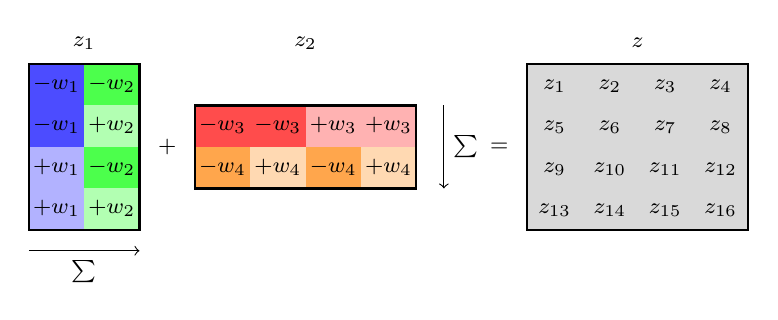
\begin{tikzpicture}[font=\footnotesize]
    \def\cw{2em}
    \def\ch{1.5em}
    
    \tikzset{cell/.style={
        inner sep=0pt,
        outer sep=0pt,
        minimum width=\cw,
        minimum height=\ch,
        align=center,
        text height=1ex,
        text depth=0.25ex,
        anchor=north west
    }}

    % 1st block
    \node[cell, fill=blue!70]   at (0*\cw, 0*\ch)  {$-w_1$};
    \node[cell, fill=blue!70]   at (0*\cw,-1*\ch)  {$-w_1$};
    \node[cell, fill=blue!30]   at (0*\cw,-2*\ch)  {$+w_1$};
    \node[cell, fill=blue!30]   at (0*\cw,-3*\ch)  {$+w_1$};
    \node[cell, fill=green!70]  at (1*\cw, 0*\ch)  {$-w_2$};
    \node[cell, fill=green!30]  at (1*\cw,-1*\ch)  {$+w_2$};
    \node[cell, fill=green!70]  at (1*\cw,-2*\ch)  {$-w_2$};
    \node[cell, fill=green!30]  at (1*\cw,-3*\ch)  {$+w_2$};
    \node                       at (\cw,0.5*\ch) {$z_1$};
    \draw[->](0,-4*\ch-0.5*\ch) -- (2*\cw,-4*\ch-0.5*\ch) node[midway,below]{$\sum$};

    \node at (2*\cw+0.5*\cw,-2*\ch) {$+$};
    
    % 2nd block
    \node[cell, fill=red!70]    at (3*\cw,-1*\ch) {$-w_3$};
    \node[cell, fill=red!70]    at (4*\cw,-1*\ch) {$-w_3$};
    \node[cell, fill=red!30]    at (5*\cw,-1*\ch) {$+w_3$};
    \node[cell, fill=red!30]    at (6*\cw,-1*\ch) {$+w_3$};
    \node[cell, fill=orange!70] at (3*\cw,-2*\ch) {$-w_4$};
    \node[cell, fill=orange!30] at (4*\cw,-2*\ch) {$+w_4$};
    \node[cell, fill=orange!70] at (5*\cw,-2*\ch) {$-w_4$};
    \node[cell, fill=orange!30] at (6*\cw,-2*\ch) {$+w_4$};
    \node                       at (5*\cw,0.5*\ch) {$z_2$};
    \draw[->](7*\cw+0.5*\cw,-1*\ch) -- (7*\cw+0.5*\cw,-3*\ch) node[midway,right]{$\sum$};

    \node at (8*\cw+0.5*\cw,-2*\ch) {$=$};

    % 3rd block
    \node[cell, fill=gray!30]    at (9*\cw,0*\ch) {$z_1$};
    \node[cell, fill=gray!30]    at (10*\cw,0*\ch) {$z_2$};
    \node[cell, fill=gray!30]    at (11*\cw,0*\ch) {$z_3$};
    \node[cell, fill=gray!30]    at (12*\cw,0*\ch) {$z_4$};
    \node[cell, fill=gray!30]    at (9*\cw,-1*\ch) {$z_5$};
    \node[cell, fill=gray!30]    at (10*\cw,-1*\ch) {$z_6$};
    \node[cell, fill=gray!30]    at (11*\cw,-1*\ch) {$z_7$};
    \node[cell, fill=gray!30]    at (12*\cw,-1*\ch) {$z_8$};
    \node[cell, fill=gray!30]    at (9*\cw,-2*\ch) {$z_9$};
    \node[cell, fill=gray!30]    at (10*\cw,-2*\ch) {$z_{10}$};
    \node[cell, fill=gray!30]    at (11*\cw,-2*\ch) {$z_{11}$};
    \node[cell, fill=gray!30]    at (12*\cw,-2*\ch) {$z_{12}$};
    \node[cell, fill=gray!30]    at (9*\cw,-3*\ch) {$z_{13}$};
    \node[cell, fill=gray!30]    at (10*\cw,-3*\ch) {$z_{14}$};
    \node[cell, fill=gray!30]    at (11*\cw,-3*\ch) {$z_{15}$};
    \node[cell, fill=gray!30]    at (12*\cw,-3*\ch) {$z_{16}$};
    \node                       at (11*\cw,0.5*\ch) {$z$};
    
    % Draw borders for the w block
    \draw[black, thick] (0,0) rectangle (2*\cw,-4*\ch);
    \draw[black, thick] (3*\cw,-1*\ch) rectangle (7*\cw,-3*\ch);
    \draw[black, thick] (9*\cw,0) rectangle (13*\cw,-4*\ch);
    
    \end{tikzpicture}
    \caption{Computation of $z$ in BIDE}
    \label{fig:z_precomputed}
\end{figure}
We can thus take advantage of this structure and isolate two blocks $z_1$ and $z_2$ such that adding all pairs of entries of $z_1$ and $z_2$ give back $z$ the pre-activation value of the neuron. Note that multiple choices of $z_1$ and $z_2$ are possible depending on the location where you split $W$.

\section{Experimental Results}
This section presents an evaluation of the SICK BIDE framework across various scenarios using our implementation of SICK. 
We first examine performance metrics for the different variants, followed by an analysis of SICK’s applicability to the modeling of continuous distributions. The results are summarized in tables and figures.

\subsection{Experimental Setup}
To evaluate the performance of SICK BIDE, we measured the execution time for two isolated settings. The first setting is a batch size of $64$ and the second is a simulation of the final layer of a transformer-based model with a batch size of $32$, a context size of $512$, and a hidden dimension of $32$.
The experiments were conducted on an NVIDIA GeForce RTX 4060 Laptop GPU, which provides:
\begin{itemize}
\item 11.61 TFLOPS of peak compute performance.
\item 256.0 GB/s of memory bandwidth.
\end{itemize}

We compared three variants in this setting:
\begin{itemize}
\item Torch implementation with automated kernel fusion: An implementation of BIDE without using any manually crafted kernel. We use torch.compile whenever we can for automated kernel fusion.
\item Bruteforce Variant: Direct computation of the integral kernel without optimizations.
\item Pre-computated Variant: Leveraging pre-computed intermediate values described in \ref{method_pre_coputation} to reduce computational overhead.
\end{itemize}
The results focus on kernel execution time, throughput, effective FLOPs, and memory bandwidth utilization.

Finally we tested sick in a practical setting, by learning an embedding for 4 distributions at the same time:
\begin{itemize}
    \item A Normal distribution with $\mu=3, \sigma=1$
    \item A Gamma distribution with $\alpha=2, \beta=1$
    \item A Mixture of two normal distributions with $p=0.2, \mu_1=120, \sigma_1=1, \mu_2=132, \sigma_2=1.5$ 
    \item a Pareto distribution with $x=1, k=1$
\end{itemize}
We run the training for $2000$ steps with batch size $64$ and using mixed precision.
This final experiment showcase the modeling power of BIDE while providing an good end to end test for the SICK kernel.

\subsection{Performance Metrics}

\subsubsection{Variant results}

\begin{table}[ht]
    \centering
    \begin{tabular}{l c S[table-format=3.2] S[table-format=3.2] S[table-format=3.2] S[table-format=3.2] S[table-format=3.2] S[table-format=3.2]}
    \toprule
    \textbf{Operation} & \textbf{Batch size} & \multicolumn{2}{c}{\textbf{torch.compile}} & \multicolumn{2}{c}{\textbf{Bruteforce}} & \multicolumn{2}{c}{\textbf{Precomputed}} \\ 
    \cmidrule(lr){3-4} \cmidrule(lr){5-6} \cmidrule(lr){7-8}
    & & \textbf{fp32} & \textbf{fp16} & \textbf{fp32} & \textbf{fp16} & \textbf{fp32} & \textbf{fp16} \\ 
    \midrule
    Normalisation constant & 64    & 11.71 & 7.09 & 0.86 & 0.69 & 0.44 & \textbf{0.36} \\
            & 16384 & {OOM}   & {OOM}  & 201.54 & 145.61 & 93.53 & \textbf{63.29} \\ 
    \midrule
    Fused cross-entropy forward & 64    & 11.72 & 6.59 & 0.88 & 0.62 & 0.45 & \textbf{0.34} \\
                                & 16384 & {OOM} & {OOM} & 199.23 & 148.43 & 91.57 & \textbf{63.48} \\ 
    \midrule
    Fused cross-entropy backward & 64    & {-}   & {-}  & \textbf{0.90} & 0.95 & 1.18 & 1.14 \\
                                 & 16384 & {OOM} & {OOM} & 235.13 & 235.06 & \textbf{227.38} & 228.73 \\ 
    \bottomrule
    \end{tabular}
    \captionsetup{justification=centering, skip=10pt} % Adjust caption spacing
    \caption{Compute time for: vanilla PyTorch implementation, bruteforce, and precomputed variants of the SICK kernel}
    \label{tab:global_results}
\end{table}
The results highlight a spectrum of computational trade-offs across implementations for all operations in Table \ref{tab:global_results}. The “torch.compile” implementation, while straightforward, is lacking memory for larger batch sizes due to its reliance on materializing full intermediate results. 
For all kernels except the backward pass we observe a significant reduce in runtime when comuting in float16 compared to float32. The precomputed variant wins in all tested cases.

In contrast, the results for the backward kernel are more mitigated. The bruteforce variant wins for the small batch sizes while the precomputed variant is prefered for heavy batch sizes but with a small margin. Furthermore we observe that the float16 computation doesn't improve significantly the kernel runtime, even degrading it sometimes.

\subsubsection{Implementation efficiency}
\begin{table}[ht]
    \centering
    \begin{tabular}{l S[table-format=3.2] S[table-format=3.2] S[table-format=3.2] S[table-format=3.2] S[table-format=3.2] S[table-format=3.2]}
    \toprule
    \textbf{Variant} & \textbf{Execution Time (ms)} & \textbf{Throughput (Hz)} & \multicolumn{2}{c}{\textbf{FLOPs (Tops/s)}} & \multicolumn{2}{c}{\textbf{Memory Bandwidth (Gb/s)}} \\
    \cmidrule(lr){4-5} \cmidrule(lr){6-7}
    & & & \textbf{Value} & \textbf{Peak FLOPS (\%)} & \textbf{Value} & \textbf{Peak Mem BW (\%)} \\ 
    \midrule
    Bruteforce & 145.61 & 6.87 & 8.29 & 71.39 & 0.12 & 0.05 \\
    Precomputed & 63.29 & 15.80 & 2.38 & 20.46 & 8.50 & 3.32 \\ 
    \bottomrule
    \end{tabular}
    \captionsetup{justification=centering, skip=10pt} % Adjust caption spacing
    \caption{Performance comparison for bruteforce and precomputed variants in fp16 with batch size 16384.}
    \label{tab:implementation_efficiency}
\end{table}

Table \ref{tab:implementation_efficiency} provides an analysis of memory and compute requirements for the integral kernel. We infer the flops and memory bandwidth based on our model described in appendix \ref{apdx:theoretical_analysis} and compare them to the theoretical figures of the GPU. As expected, the precomputed variant utilizes less computational power but demanded more memory bandwidth compared to the bruteforce implementation.

Despite leveraging more than 70\% of the GPU's theoretical max computing power the bruteforce variant is more than 2x slower than the precomputed one.

While it is clear that the bruteforce kernel is saturated by heavy computing pipelines utilization, we note that out implementation of the precomputed kernel struggle to fully utilize the potential of the GPU.

\subsection{Modeling Continuous Distributions}
We also evaluated SICK on a practical example end to end to assess for its viability

\begin{table}[ht]
    \centering
    \begin{tabular}{l S[table-format=2.2] S[table-format=1.6] S[table-format=3.2]}
    \toprule
    \textbf{Method} & \textbf{Runtime (s)} & \textbf{Train Loss (EMA)} & \textbf{Peak Memory (MB)} \\ 
    \midrule
    Vanilla & 37.38 & 7.227091 & 418.42 \\ 
    Bruteforce & 6.88 & 7.256562 & 163.43 \\ 
    Precompute & 7.62 & 7.195776 & 163.43 \\ 
    \bottomrule
    \end{tabular}
    \captionsetup{justification=centering, skip=10pt} % Adjust caption spacing
    \caption{Comparison of runtime, loss (EMA), and peak memory usage for Vanilla, Bruteforce, and Precompute methods.}
    \label{tab:method_comparison}
\end{table}

The vanilla method, while straightforward, suffered from excessive runtime and memory overhead. In contrast, both the bruteforce and precomputed variants significantly reduced both memory usage and runtime, demonstrating the efficiency of SICK BIDE while reaching a comparable train loss.

\begin{figure}[ht]
    \centering
    \includegraphics[width=1\textwidth]{continuous_distribution_estimations.png}
    \captionsetup{justification=centering} % Adjust caption spacing
    \caption{Continuous distribution estimations using SICK BIDE.}
    \label{fig:continuous_distribution}
\end{figure}

Figure \ref{fig:continuous_distribution} shows the obtained cdfs and density functions for the precompute variant compared to the true cdfs and densities. We observe that the CDFs match closely their targets. The Pareto CDF is a bit off for values close to one.
For the densities however we can note some disparities:
\begin{itemize}
    \item For the Normal distribution we see some perturbations around zero (probably because the concentration of float16 numbers is higher at this spot)
    \item For the Gamma distribution the tip is a bit off and some of the probability mass ends up in negative numbers which is theoretically impossible for a gamma distribution but can be attributed to approximations artifacts.
    \item For the Mixture of normales the tip of the stronger normal component is a bit off
    \item For the Pareto distribution we observe that what should be a density going to infinity the closest it get to zero at some point go back to zero in practice. This is to be expected as BIDE's density function is defined over the full float16 set and thus include impossible values such as negative ones for which the theoretical density should be zero.  
\end{itemize}

\subsection{Insights}
\begin{itemize}
    \item Trade-Off Analysis: The precomputed variant manage to significantly reduce the runtime of the kernel. The bruteforce variant achieved an honorable runtime by  extracting most of the GPU's computing capacity.
    \item Practical Applicability: SICK BIDE effectively handled continuous distributions and approximated well the theoretical densities
    \item Integration Potential: The framework’s GPU-optimized nature makes it well-suited for integration into modern AI systems.
\end{itemize}

In summary, SICK BIDE demonstrates strong potential as a scalable and efficient solution for complex distribution modeling. Future optimizations in hardware, algorithm design, and implementations will further enhance its viability across a broader range of applications.

\section{Discussion}
The results and analyses presented in this paper highlight the practical and theoretical potential of the SICK BIDE framework for distribution modeling. Below, we discuss key insights, trade-offs, limitations, and avenues for future exploration.

\subsection{Limitations of Current Optimizations}
Despite the gains achieved through pre-computation, several limitations remain:
\begin{itemize}
    \item Implementation: Our implementation utilizes triton which is a DSL and still under development. We know from our theoretical analysis that the overhead of our implementation prevent the kernel to fully utilize all the performances of the GPU. Maybe a better triton implementation or even a CUDA implementation could reach better computing resources utilization.
    \item Modeling precision: Our experiments showed that BIDE can match quite well the theoretical distributions, but not perfectly. There are probably other implicit representations that could better model the theoretical distributions and match the performances of non assumption-free methods. 
    \item Number of bits: The current implementation of BIDE allow to represent distributions over 16bits numbers in a LLM-like setting (reasonable batch size * context size). However to be able to fully represent UTF-8 encoded text, we need to upgrade BIDE to 64bits numbers. This is out of the reach of the current state of development of BIDE but could change in the future with both software and hardware innovations. 
\end{itemize}

\subsection{Opportunities for Future Optimizations}
To address these limitations, several strategies warrant exploration:

\begin{itemize}
\item Hierarchical Decomposition: Other hierarchical decompositions methods could improve scalability, leveraging effectively patterns in binary combinations inputs.
\item Lower-Precision Computing: Integrating low-precision approaches could balance memory and computational efficiency by leveraging modern low-precision hardware features, viabilizing the approach for BIDE with higher number of bits.
\item Moore's law: As the GPUs become more performant with time, the SICK BIDE framework designed to maximaly use computing ressources will directly benefit from hardware advances and become naturally viable for higher numbers of bits as time passes.
\end{itemize}

\section{Conclusion and Future Work}
In this paper, we introduced Binary Implicit Distribution Encoding (BIDE) and the Softmax Integral Compute Kernel (SICK) as a novel paradigm for assumption-free distribution modeling by directly leveraging binary representations. By focusing on binary encoding, BIDE enables the modeling of both categorical and continuous distributions with high expressiveness and efficiency. SICK, a GPU-optimized kernel, complements this framework by making the computation of the softmax normalization constants tractible, avoiding approximations.

Our theoretical and experimental analysis demonstrated the feasibility of integrating SICK BIDE into modern machine learning pipelines, to efficiently model conditional distributions over vocabulary or real numbers. We provided a comprehensive breakdown of memory and computational requirements, showing that the approach achieves competitive GPU throughput. The empirical results on an NVIDIA GeForce RTX 4060 Laptop GPU validate these trade-offs, offering practical insights into kernel optimization for real-world deployment.

Despite its strengths, this work highlights areas for further improvement. For example, while the pre-computation strategy mitigates the computational overhead, its current implementation struggles to utilize GPUs to their full capabilities. Moreover, as the current implementation relies heavily on GPU compute capacity, optimizing SICK BIDE for other hardware accelerators (e.g., TPUs or custom ASICs) could unlock additional performance gains.

Looking ahead, several exciting directions emerge for future research. These include:
\begin{itemize}
\item Hierarchical and Approximation Techniques: Developing hierarchical computation strategies or approximation methods to further reduce memory and FLOP requirements without sacrificing accuracy.
\item Mixed-Precision and Quantization: Exploring lower-precision or quantized computation for SICK to improve efficiency on resource-constrained devices.
\item Broader Application Domains: Extending BIDE to other domains, such as becoming an LLM's output layer
\item Integration with AI Frameworks: Seamlessly integrating SICK BIDE into popular AI frameworks like PyTorch or TensorFlow, making it accessible to a broader audience.
\item Scaling Beyond Current Constraints: Investigating ways to handle higher input dimensions or batch sizes by leveraging distributed GPU computation or advanced memory management techniques.

In conclusion, the BIDE and SICK framework represents a significant step forward in leveraging binary representations for efficient assumption-free distribution modeling. By combining theoretical rigor with practical innovations, we hope this work inspires further exploration and application of binary-based neural architectures in diverse machine learning and AI challenges.
\end{itemize}

\section*{Acknowledgments}
This was was supported in part by......

%Bibliography
\bibliographystyle{unsrt}  
\bibliography{references}  

\appendix
\section{Notations}
Numbers:
\begin{itemize}
\item $B$: Number of bits of BIDE
\item $H$: Hidden size of BIDE
\item $F$: Element size of BIDE dtype
\item $\mathcal{B}$: Batch size
\item $\mathcal{K}$: Input dimension ($2^B$)
\item $N$: Batch dimension block size
\item $K$: Input dimension block size
\end{itemize}

BIDE Tensors:
\begin{itemize}
\item $W$: Weights of BIDE 1st layer, shape $(N, H, B)$
\item $r$: Weights of BIDE 2nd layer, shape $(N, H)$
\item $b$: input values represented as bits mapped to $\{-1, 1\}$., shape $(N, K, B)$
\item $z$: intermediate values of BIDE, shape $(N, K, H)$
\item $h$: activations of BIDE's hidden layer, shape $(N, K, H)$
\item $l$: logits (output) of BIDE, shape $(N, K)$
\item $m$: max logit of BIDE, shape $(N)$
\item $s$: sum of the exponential of the logits (normalization constant), shape $(N)$
\item $p$: probabilities of BIDE, shape $(N, K)$
\end{itemize}

Precomputed Tensors:
\begin{itemize}
    \item $\tilde{K}=2^{\frac{\log_2{K}}{2}}=\sqrt{2^{log_2{K}}}=\sqrt{K}$: the number of combinations of inputs for half the bits of BIDE.
    \item $\tilde{b}_1$ and $\tilde{b}_2$: Respectively the first and last half of the input bits representation
    \item $\tilde{z}_1$ and $\tilde{z}_2$: The intermediate values of BIDE computed over respectively $\tilde{b}_1$ and $\tilde{b}_2$

\end{itemize}

\section{Theoretical Analysis for SICK} \label{apdx:theoretical_analysis}
\subsection{Bruteforce-variant}
Memory:
\begin{itemize}
    \item Load $W$: $FNHB$
    \item Load $r$: $FNH$
    \item Write $m$: $FN$
    \item Write $s$: $FN$
\end{itemize}

Total: $FN(H(B+1)+2)$

Compute:
\begin{itemize}
    \item Compute $b$ (>>, \&, fma): $KB3$
    \item Compute $z$ (gemm): $NKHB2$
    \item Compute $h$ (relu): $NKH$
    \item Compute $l$ (gemm): $NKH2$
    \item Compute $m$ (max): $NK$
    \item Compute $s$ (-m, exp, sum): $NK3$
\end{itemize}

Total: $K(3B+N(H(B2+3)+4))$

\subsection{Precomputed-variant}
\begin{itemize}
    \item Load $\tilde{z}_1$: $FNH\tilde{K}$
    \item Load $\tilde{z}_2$: $FNH\tilde{K}$
    \item Load $r$: $FNH$
    \item Write $m$: $FN$
    \item Write $s$: $FN$
\end{itemize}

Total: $FN(H(2^{B/2+1}+1)+2)$

Compute:
\begin{itemize}
    \item Compute $b1$ (>>, \&, fma): $\tilde{K}B3$
    \item Compute $b2$ (>>, \&, fma): $\tilde{K}B3$
    \item Compute $\tilde{z}_1$ (gemm): $N\tilde{K}HB2$
    \item Compute $\tilde{z}_2$ (gemm): $N\tilde{K}HB2$
    \item Compute $z$ (+): $NKH$
    \item Compute $h$ (relu): $NKH$
    \item Compute $l$ (gemm): $NKH2$
    \item Compute $m$ (max): $NK$
    \item Compute $s$ (-m, exp, sum): $NK3$
\end{itemize}

Total: $6\tilde{K}B+N(4\tilde{K}HB+K(4H+4))$

\subsection{Numerical application}
We would like to estimate the throughput needed to viably run BIDE on a device. One particular use case that interests us is the use of BIDE as a LLM head.\
In particular let's consider as a baseline the \href{https://github.com/karpathy/nanoGPT}{nano-gpt repository} which is a minimalistic implementation of GPT-2.\
Training this type of model on modern GPUs with mixed precision, we can expect roughly that the final layer + loss computation should be in the order of $10ms$ for a batch size of $32$ with a context size of $512$.\
If we want to use BIDE as a LLM head (either to serve as an implicit distribution over tokens or over a real number) we would like a reasonable precision like at least 16 bits.\
For this setting to be viable we can ask the simple question:\
How many memory bandwidth / FLOPs are required to run 16bits-BIDE with batch size $32$ such that the loss computation in float16 is ~$10ms$?
\begin{itemize}
    \item $B=16$
    \item $H=32$ (2x the input size, default setting)
    \item $\mathcal{B}=32*512=16384$
    \item $\mathcal{K}=2^B=65536$
    \item $F=2$
\end{itemize}

\begin{table}[ht]
\centering
\begin{tabular}{|l|c|c|}
\hline
\textbf{Tensor/Operation} & \textbf{Bruteforce Variant} & \textbf{Precomputed Variant} \\ \hline
Load $W$ & $16.78$ Mb & - \\ \hline
Load $r$ & $1.05$ Mb & $1.05$ Mb \\ \hline
Load $\tilde{z}_1$ & - & $268.44$ Mb \\ \hline
Load $\tilde{z}_2$ & - & $268.44$ Mb \\ \hline
Write $m$ & $32.77$ kb & $32.77$ kb \\ \hline
Write $s$ & $32.77$ kb & $32.77$ kb \\ \hline
\textbf{Total} & $17.89$ Mb & $537.99$ Mb \\ \hline
\textbf{Required bandwidth} & 1.79GB/s & 53.8GB/s \\ \hline
\end{tabular}
\caption{Comparison of Memory Requirements for Bruteforce and Precomputed Variants.}
\label{table:variants-comparison}
\end{table}

\begin{table}[ht]
\centering
\begin{tabular}{|l|c|c|}
\hline
\textbf{Tensor/Operation} & \textbf{Bruteforce Variant} & \textbf{Precomputed Variant} \\ \hline
Compute $b$ & $3.15$ Mops & - \\ \hline
Compute $b1$ & - & $12.29$ kops \\ \hline
Compute $b2$ & - & $12.29$ kops \\ \hline
Compute $z$ & $1.1$ Tops & $34.36$ Gops \\ \hline
Compute $\tilde{z}_1$ & - & $4.29$ Gops \\ \hline
Compute $\tilde{z}_2$ & - & $4.29$ Gops \\ \hline
Compute $h$ & $34.36$ Gops & $34.36$ Gops \\ \hline
Compute $l$ & $68.72$ Gops & $68.72$ Gops \\ \hline
Compute $m$ & $1.07$ Gops & $1.07$ Gops \\ \hline
Compute $s$ & $3.22$ Gops & $3.22$ Gops \\ \hline
\textbf{Total} & $1.21$ Tops & $150.32$ Gops \\ \hline
\textbf{Required capacity} & 120.69TFLOPs & 15.03TFLOPs \\ \hline
\end{tabular}
\caption{Comparison of Memory and Compute Requirements for Bruteforce and Precomputed Variants.}
\label{table:variants-comparison}
\end{table}

\section{Formula for backward pass} \label{appendix_backward_pass}

\subsection*{Notation}

\begin{itemize}
    \item $\mathcal{L}$: Loss function 
    \item $n$, $N$: index of the minibatch example and number of examples in the minibatch.
    \item $k$ and $K$: index of the binary input value and number of binary input combinations.
    \item $b_{kj}$: representation of bit $j$ (-1 if the bit is 0, else 1) for the $k$-th binary input value
    \item $W$: weights of the first layer of the BIDE MLP
    \item $r$: weights of the second layer of the BIDE MLP
    \item $h_{ki}$: value of the $i$-th hidden unit for the $k$-th binary input value
    \item $l_{k}$: logit of the $k$-th binary input value
    \item $p_{k}$: probability of the $k$-th binary input value
    \item $y_n$: index of the target value for the $n$-th example
    \item $\delta_{ky_n}$: Kronecker delta, equal to 1 if $k = y_n$ and 0 otherwise
    \item $m$: maximum value of the logits (used for softmax numerical stability)
    \item $s$: sum of the exponentials of the logits (used for softmax normalization)
\end{itemize}

\subsection*{Calculations}

We want to compute $\frac{\partial \mathcal{L}}{\partial r}$ and $\frac{\partial \mathcal{L}}{\partial W}$ in an efficient way. Here are the calculations assuming mean reduction for the loss over the minibatch:

\subsection*{Gradient of $r$}
\[
\begin{aligned}
\frac{\partial \mathcal{L}}{\partial r_i} &= \frac{1}{N} \sum_{n=1}^{N} \sum_{k=1}^{K} \frac{\partial l_k}{\partial r_i} \frac{\partial \mathcal{L}}{\partial l_k} \\
&= \frac{1}{N} \sum_{n=1}^{N} \sum_{k=1}^{K} h_{ki} (p_k - \delta_{ky_n}) \\
&= \frac{1}{N} \sum_{n=1}^{N} \left( \sum_{k=1}^{K} h_{ki} p_k - \sum_{k=1}^{K} h_{ki} \delta_{ky_n} \right) \\
&= \sum_{k=1}^{K} h_{ki} p_k - \frac{1}{N} \sum_{n=1}^{N} h_{y_ni} \\
&= \sum_{k=1}^{K} h_{ki} \frac{\exp(l_k - m)}{s} - \frac{1}{N} \sum_{n=1}^{N} h_{y_ni} \\
&= \frac{1}{s} \sum_{k=1}^{K} h_{ki} \exp(l_k - m) - \frac{1}{N} \sum_{n=1}^{N} h_{y_ni} \\
\end{aligned}
\]

\subsection*{Gradient of $W$}
\[
\begin{aligned}
\frac{\partial \mathcal{L}}{\partial W_{ij}} &= \frac{1}{N} \sum_{n=1}^{N} \sum_{k=1}^{K} \frac{\partial h_{ki}}{\partial W_{ij}} \frac{\partial l_k}{\partial h_{ki}} \frac{\partial \mathcal{L}}{\partial l_k} \\
&= \frac{1}{N} \sum_{n=1}^{N} \sum_{k=1}^{K} b_{kj} \mathbbm{1}_{h_{ki} > 0} r_i (p_k - \delta_{ky_n}) \\
&= \frac{1}{N} \sum_{n=1}^{N} \left( \sum_{k=1}^{K} b_{kj} \mathbbm{1}_{h_{ki} > 0} r_i p_k - \sum_{k=1}^{K} b_{kj} \mathbbm{1}_{h_{ki} > 0} r_i \delta_{ky_n} \right) \\
&= \sum_{k=1}^{K} b_{kj} \mathbbm{1}_{h_{ki} > 0} r_i p_k - \frac{1}{N} \sum_{n=1}^{N} b_{y_nj} \mathbbm{1}_{h_{y_ni} > 0} r_i \\
&= \sum_{k=1}^{K} b_{kj} \mathbbm{1}_{h_{ki} > 0} r_i \frac{\exp(l_k - m)}{s} - \frac{1}{N} \sum_{n=1}^{N} b_{y_nj} \mathbbm{1}_{h_{y_ni} > 0} r_i \\
&= \frac{1}{s} \sum_{k=1}^{K} b_{kj} \mathbbm{1}_{h_{ki} > 0} r_i \exp(l_k - m) - \frac{1}{N} \sum_{n=1}^{N} b_{y_nj} \mathbbm{1}_{h_{y_ni} > 0} r_i \\
\end{aligned}
\]

\end{document}
